% !TeX spellcheck = en_US

\documentclass[document.tex]{subfiles}

\begin{document}
    \section{Anomaly Detection}
    
    \subsection{Definitions}    

    \begin{frame}{Anomalies and Anomaly Detection}
        \begin{columns}
            \begin{column}{0.6\textwidth}
                \begin{itemize}
                    \item When there are \textbf{patterns} in data that \textbf{do not conform} to a well defined notion of \textbf{normal behavior}, those patterns are commonly referred to as \textbf{anomalies}.
                    \item Such patterns might be induced in the data for a variety of reasons, such as \textbf{malicious activity}, e.g., credit card fraud, cyber-intrusion, terrorist activity or breakdown of a system.
                    \item Anomalies in data translate to \textbf{significant and often critical actionable information} that call for more \textbf{attention} or \textbf{investigation} - usually \textbf{signaling} a change in the \textbf{underlying conditions}.
                    \item The \textbf{identification} of unusual patterns that do not conform to expected behavior is the primary goal of \textbf{anomaly detection} for which various techniques exist.
                \end{itemize}
            \end{column}
            \begin{column}{0.4\textwidth}
                \begin{figure}
                    \label{fig:anomalies}
                    \includegraphics[width=\textwidth]{figures/anomalies.pdf}
                \end{figure}
            \end{column}
        \end{columns}
    \end{frame}
    
    \begin{frame}{Anomaly Types}
        \begin{alertblock}{\textsc{Point anomalies}}
            A \textbf{data instance} is anomalous if it's \textbf{too far away} from the \textbf{rest of the data}, For example, a single purchase might be an anomalous transaction when the transaction value is large with respect to the rest of all other transactions.
        \end{alertblock}
        \begin{alertblock}{\textsc{Contextual anomalies}}
            A \textbf{data instance} is anomalous \textbf{only in a specific context} but not otherwise, which is a commony type of anomaly in time-series data. For example, a network intrusion system might flag large spikes in network traffic at the middle of the night as anomalous behavior.
        \end{alertblock}
        \begin{alertblock}{\textsc{Collective anomalies}}
            Collective anomalies are \textbf{collections of related data instances} that are anomalous with respect to the entire dataset, but not individual values. Those anomalies are for example events in an unexpected order (e.g., breaking rhythm in ECG) or unexpected value combinations (e.g., buying a large number of expensive items).
        \end{alertblock}
    \end{frame}
    
    \begin{frame}{Un-/Supervised Anomaly Detection}
        \begin{itemize}
        \item When there is \textbf{labeled training data}, \textbf{balance between anomalous and normal classes} and the \textbf{data is not autocorrelated}, then there is \textbf{no need for anomaly detection} techniques as \textbf{supervised machine learning models} like random forests or support vector machines can do the job.
        \item However, in most \textbf{labeled training datasets} there will be a \textbf{few dozen anomalies} among \textbf{millions of regular data points}. Supervised machine learning algorithms will \textbf{classify} almost all \textbf{data as normal} because doing so will provide a \textbf{very high accuracy} score. Nevertheless, this problem can be solved by \textbf{resampling techniques} that we'll in the forthcoming chapter.
        \item A problem that is not solvable is the problem of \textbf{autocorrelation}, which means that one \textbf{data point does depend on an earlier data point}, which is far more \textbf{common in time-series data} and thus \textbf{simple classifier would not work well}.
        \item \textbf{Without labeled training data}, methods from \textbf{unsupervised learning} can accomplish anomaly detection tasks. However, as there is \textbf{no test data}, it is \textbf{not possible} to find out h\textbf{ow well the model is doing}. Hence, the results of those methods need to be \textbf{tested in the field} before placing them in the critical path.
        \end{itemize}
    \end{frame}
    
    \begin{frame}{Anomaly Detection Techniques}
        \begin{alertblock}{\textsc{Statistical-based Anomaly Detection}}
        Statistical methods try to identify anomalies in data by flagging those data instances that \textbf{deviate from common statistical properties of a distribution}, including mean, median, mode, and quantiles.
        \end{alertblock}
    
        \begin{alertblock}{\textsc{Clustering-Based Anomaly Detection}}
            The assumption in clustering-based anomaly detection is that \textbf{data instances that are similar} tend to belong to \textbf{similar groups or clusters}, as determined by their \textbf{distance from local centroids}. Algorithms: k-Means.
        \end{alertblock}
    
        \begin{alertblock}{\textsc{Density-Based Anomaly Detection}}
        The assumption in density-based anomaly detection is that a normal \textbf{data instances occur around a dense neighborhood} and abnormalities are far way. Algorithms: k-nearest neighbor (k-NN), local outlier factor (LOF).
        \end{alertblock}
    \end{frame}

    \subsection{Statistical-Based Anomaly Detection}

    \begin{frame}{Introductory Example I/II}
        In the following we will be using a dataset which contains the number of \textbf{daily passengers in yellow taxi cabs} in New York City between \textbf{2014-07-01 and 2015-01-31}.
        \begin{figure}
            \label{taxi-passengers-visualization}
            \includegraphics[width=\textwidth]{figures/taxi-passengers-visualization.pdf}
        \end{figure}
        With the data given, we now want to \textbf{detect historical anomalies} in this time series in an \textbf{automated manner} and try to find \textbf{explanations for their occurence}. \href{https://nbviewer.jupyter.org/github/saschaschworm/big-data-and-data-science/blob/master/notebooks/demos/taxi-passengers-low-pass-filter.ipynb}{\textsc{\textbf{$\rightarrow$ open notebook in nbviewer}}}
    \end{frame}
    
    \begin{frame}{Moving Average/Low Pass Filter}
        \begin{itemize}
            \item A \textbf{time series}, that is a \textbf{sequence of numerical data points in successive order} like in our taxi passengers dataset here, is a good example of \textbf{contextual} and \textbf{collective anomalies} in a \textbf{univariate dataset} and a simple way to find those is to flag data points that deviate from common statistical properties of a distribution, e.g. mean, median, mode and quantiles.
            \item For our example here, we define an anomaly as a \textbf{data point in the time series that deviates by 3 standard deviations from the mean} but as the \textbf{mean is not static over time} we need a \textbf{rolling window} to compute the average across the data time.
            \item This process is called \textbf{moving average} or \textbf{low pass filter} which calculates the means of the actual data in \textbf{small batches} and thus \textbf{smooths short-term fluctuations and highlights long-term} ones which in turn results into a \textbf{general movement} of data over time called \textbf{trend}.
            \item Finding anomalies this way therefore means to calculate a \textbf{moving average} as well as a \textbf{moving standard deviation} and apply the \textbf{three-sigma rule} which serves as a \textbf{threshold}. So in our case, whenever an actual \textbf{data point is higher or lower than 3 standard deviations of the moving average} in a window of lets say \textbf{20 days} we will flag this data point as an anomaly.
        \end{itemize}
    \end{frame}
    
    \begin{frame}{Python Implementation: Moving Average/Low Pass Filter}
        \lstinputlisting[language=Python, style=material]{snippets/taxi-passengers-low-pass-1.py}
    \end{frame}

    \begin{frame}{Moving Average/Low Pass Filter Visualization}
        \begin{figure}
            \label{fig:taxi-passengers-low-pass}
            \includegraphics[width=\textwidth]{figures/taxi-passengers-low-pass.pdf}
        \end{figure}
    \end{frame}

    \begin{frame}{Python Implementation: Moving Average/Low Pass Filter Anomaly Detection}
        \lstinputlisting[language=Python, style=material]{snippets/taxi-passengers-low-pass-2.py}
    \end{frame}

    \begin{frame}{Python Implementation: Moving Average/Low Pass Filter Anomaly Detection Visualization}
        \begin{figure}
            \label{fig:taxi-passengers-low-pass-result}
            \includegraphics[width=\textwidth]{figures/taxi-passengers-low-pass-result.pdf}
        \end{figure}
    \end{frame}

    \stepcounter{openexercise}
    \begin{frame}{Open Exercise \arabic{openexercise}}
        The anomaly found on December 25th, 2014 is reasonable as in the United States Christmas is primary celebrated on that day and therefore many people stayed home with their families instead of driving around with taxis. But what has happened on the 26th and 27th of January 2015? Find out!
        
        \note{
            \begin{columns}
                \begin{column}{.6\textwidth}
                    \begin{justify}
                        \textit{"New York City was spared from the worst of a snowstorm that hit the Northeast early Tuesday, with the dire warnings that it could be one of the worst blizzards in the city’s history failing to materialize. [...] Mr. de Blasio took the unusual step of \textbf{ordering all drivers off the streets by 11 p.m. on Monday}, a ban that he said covered 'anything that has to do with leisure or convenience,' including, to the chagrin of many housebound New Yorkers, food delivery. The call to \textbf{completely clear the streets} was a reflection of how seriously public officials were taking the threat of the storm, which was expected to affect a 250-mile stretch of the Northeast."}
                    \end{justify}
                    The New York Times, \href{https://www.nytimes.com/2015/01/27/nyregion/new-york-blizzard.html?_r=0}{New York City Is Spared the Worst Effects of Snowstorm}, 2015
                \end{column}
                \begin{column}{.4\textwidth}
                    \begin{figure}
                        \label{fig:blizzard}
                        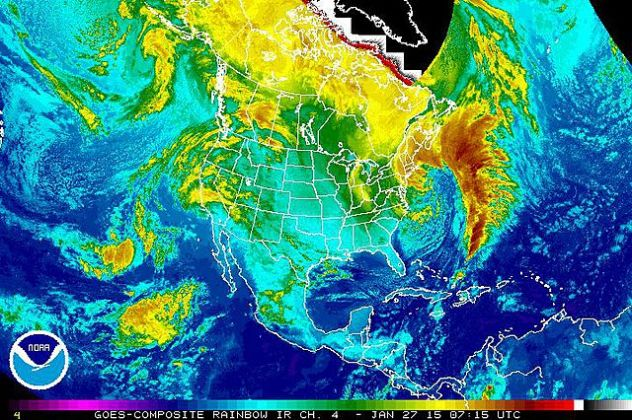
\includegraphics[width=\textwidth]{figures/external/blizzard.jpg}
                    \end{figure}
                \end{column}
            \end{columns}
        
        }
    \end{frame}

    \begin{frame}{Introductory Example II/II}
        The data we will be now taking a look on, is a another time series which contains the \textbf{monthly totals of international airline passengers} in thousands between 1949 and 1960.
        
        \begin{figure}
            \label{airline-passengers-visualization}
            \includegraphics[width=\textwidth]{figures/airline-passengers-visualization.pdf}
        \end{figure}
    
        What is easy to see here is that the data has both an \textbf{upward trend} and \textbf{seasonal variations}. At first glance, anomalies are visually not detectable but nevertheless we try to find some. \href{https://nbviewer.jupyter.org/github/saschaschworm/big-data-and-data-science/blob/master/notebooks/demos/airline-passengers-stl.ipynb}{\textsc{\textbf{$\rightarrow$ open notebook in nbviewer}}}
    \end{frame}

    \begin{frame}{Trend and Seasonality}
        \begin{itemize}
            \item A \textbf{trend} is defined as a \textbf{continuous increase or decrease} in a metrics value whereas \textbf{seasonality} is defined as \textbf{periodic or cyclical patterns} in that repeatedly occur with a fixed period of time.
            \item Time series with a trend component are \textbf{not stable or stationary} over time which means that there is \textbf{no single value for a mean} and therefore a setting a \textbf{fixed threshold} is a bad idea. For example a time series with an increasing trend, is guaranteed to eventually exceed the upper threshold limit.
            \item That is why we have been calculating a \textbf{low pass filter} which actually returns the \textbf{underlying trend component} of the time series and we then used this trend component in combination with the three-sigma rule to obtain a \textbf{dynamic threshold} for detecting anomalous data points.
            \item \textbf{Seasonality} has very \textbf{similar effects as trend} because if you would zoom into a time series with seasonality it looks like trend which makes seasonality basically a \textbf{variable trend}.
            \item Both trend and seasonality are two \textbf{major characteristics of time series} and must be handled carefully in any anomaly detection model in order to obtain the \textbf{real global anomalies} instead of finding only the unusable local ones.
        \end{itemize}
    \end{frame}

    \begin{frame}{Moving Average/Low Pass Filter Benchmark}
        When applying anomaly detection on the air passengers dataset with a low pass filter on the dataset we can clearly see that the \textbf{trend component (expressed as the orange line) has an upward direction}. It is also reasonable that the \textbf{number of airline passengers in summer is higher} compared to the other seasons.
        
        \begin{figure}
            \label{fig:airline-passengers-low-pass}
            \includegraphics[width=\textwidth]{figures/airline-passengers-low-pass-anomalies.pdf}
        \end{figure}
        \vspace*{-2mm}
         The low pass filter approach we have been using so far is \textbf{not capable of capturing the variable trend} and therefore flags data points in the summer as anomalies. Hence, we have to use method which also addresses the \textbf{seasonal component (variable trend component)} within the time series.
    \end{frame}

    \begin{frame}{Seasonal and Trend Decomposition}
        The mathematical procedure of \textbf{transforming a time series into multiple different time series} is called \textbf{time series decomposition} and involves splitting it into \textbf{3 components} called \textbf{trend, seasonal and remainder component} in the form of
        
        $$Y(t) = T(t) + S(t) + R(t)$$
        
        for an \textbf{additive decomposition} and
        
        $$Y(t) = T(t) \cdot S(t) \cdot R(t)$$
        
        for a \textbf{multiplicative decomposition} where $Y(t)$ is the value of the time series at time $t$, $T(t)$ is the trend component at time $t$ and $S(t)$ is the seasonal component at time $t$. $R(t)$ is the remainder component at time $t$ which is the \textbf{result of removing the trend and seasonal component} from the original time series.
    \end{frame}

    \begin{frame}{Seasonal and Trend Decomposition Visualization}
        \begin{figure}
            \label{fig:airline-passengers-stl}
            \includegraphics[width=\textwidth]{figures/airline-passengers-stl.pdf}
        \end{figure}
    \end{frame}

    \begin{frame}{Additive/Multiplicative Decomposition}
        \begin{columns}
            \begin{column}{.6\textwidth}
                \begin{itemize}
                    \item To achieve successful decomposition, it is important to choose between the \textbf{additive and multiplicative} models, which requires analyzing the series beforehand.
                    \item If the \textbf{seasonal variation looks constant} and does not change over time, which means it does not change when the time series value increases, an \textbf{additive model} should be used for decomposition.
                    \item If in turn the \textbf{time series increases in magnitude} and thus the \textbf{seasonal variation increases} as well, a \textbf{multiplicative model} is more appropriate.
                \end{itemize}
            \end{column}
            \begin{column}{.4\textwidth}
                \begin{figure}
                    \label{fig:additive-multiplicative-decomposition}
                    \includegraphics[width=\textwidth]{figures/additive-multiplicative-decomposition.pdf}
                \end{figure}
            \end{column}
        \end{columns}
    \end{frame}

    \begin{frame}{Python Implementation: Seasonal and Trend Decomposition}
        \lstinputlisting[language=Python, style=material]{snippets/air-passengers-stl-1.py}
    \end{frame}

    \begin{frame}{Python Implementation: Seasonal and Trend Decomposition Anomaly Detection}
        \lstinputlisting[language=Python, style=material]{snippets/air-passengers-stl-2.py}
    \end{frame}
    
    \begin{frame}{Seasonal and Trend Decomposition Anomaly Detection Visualization I/II}
        \begin{figure}
            \label{fig:airline-passengers-stl-resid-anomalies}
            \includegraphics[width=\textwidth]{figures/airline-passengers-stl-resid-anomalies.pdf}
        \end{figure}
    \end{frame}

    \begin{frame}{Seasonal and Trend Decomposition Anomaly Detection Visualization II/II}
        \begin{figure}
            \label{fig:airline-passengers-stl-anomalies}
            \includegraphics[width=\textwidth]{figures/airline-passengers-stl-anomalies.pdf}
        \end{figure}
    \end{frame}
   
    \subsection{Density-Based Anomaly Detection}
    
    \begin{frame}{Introductory Example}
        In the following example we want to find \textbf{anomalies in bank transactions} and assume that we have the following data on how many \textbf{monthly transactions} a bank customer has made in the \textbf{past 24 months} and what the \textbf{total sum} each has been.
        
        \begin{figure}
            \label{fig:lof-transactions}
            \includegraphics[width=\textwidth]{figures/lof-transactions.pdf}
        \end{figure}
    
        None of the features clearly show anomalies and thus making the methods we have been using so far inappropriate. Hence we need a \textbf{method that regards both features} at once and takes care of the \textbf{local neighborhoods} of each data point. \href{https://nbviewer.jupyter.org/github/saschaschworm/big-data-and-data-science/blob/master/notebooks/demos/transactions-lof.ipynb}{\textsc{\textbf{$\rightarrow$ open notebook in nbviewer}}}
    \end{frame}

    \begin{frame}{Local Outlier Factor (LOF)}
        \begin{columns}
            \begin{column}{0.6\textwidth}
                \begin{itemize}
                    \item When data has \textbf{multiple reading} but not a specific \textbf{order} like in time-series, one approach to identify anomalies is to use a \textbf{density-based anomaly detection technique} like the \textbf{Local Outlier Factor (LOF)}. 
                    \item LOF measures the \textbf{local density deviation} of a data point with respect to its neighbors obtained from a \textbf{k-nearest neighbor} and calculates the ratio of the \textbf{average local density} of its $k$-nearest neighbors and its \textbf{own local density}.
                    \item The \textbf{LOF value of less than 1} is an indicator that the observation is \textbf{not an outlier}, while a value \textbf{greater than 1 indicates an outlier}. The cut-off can be higher if the data is sparse.
                \end{itemize}
            \end{column}
            \begin{column}{0.4\textwidth}
                \begin{figure}
                    \label{fig:lof-transactions-combined}
                    \includegraphics[width=\textwidth]{figures/lof-transactions-combined.pdf}
                \end{figure}
            \end{column}
        \end{columns}
    \end{frame}

    \begin{frame}{Python Implementation: Local Outlier Factor Anomaly Detection}
        \lstinputlisting[language=Python, style=material]{snippets/transactions-lof.py}
    \end{frame}

    \begin{frame}{Local Outlier Factor Anomaly Detection Visualization}
        \begin{figure}
            \label{fig:lof-transactions-visualization}
            \includegraphics[width=\textwidth]{figures/lof-transactions-viz.pdf}
        \end{figure}
    \end{frame}

    \stepcounter{devexercise}
    \begin{frame}{Development Exercise \arabic{devexercise}}
        \begin{alertblock}{\textsc{Task}}
            Import the \textbf{intrusion detection dataset} \textit{(datasets $\rightarrow$ exercises $\rightarrow$ intrusion-detection.csv)} and apply the various anomaly detection techniques we have learned.
        \end{alertblock}
        \begin{alertblock}{\textsc{Question}}
            Where do anomalies occur?
        \end{alertblock}
    \end{frame}

\end{document}